As explained in Section~\ref{sec:intro} OpenMP 4.0 provides two environment variables OMP\_PROC\_BIND and OMP\_PLACES to help users define the thread placement for their shared memory OpenMP application which together we refer to as \textit{OpenMP Affinity}.%
\begin{figure}[h!]
  \centering
  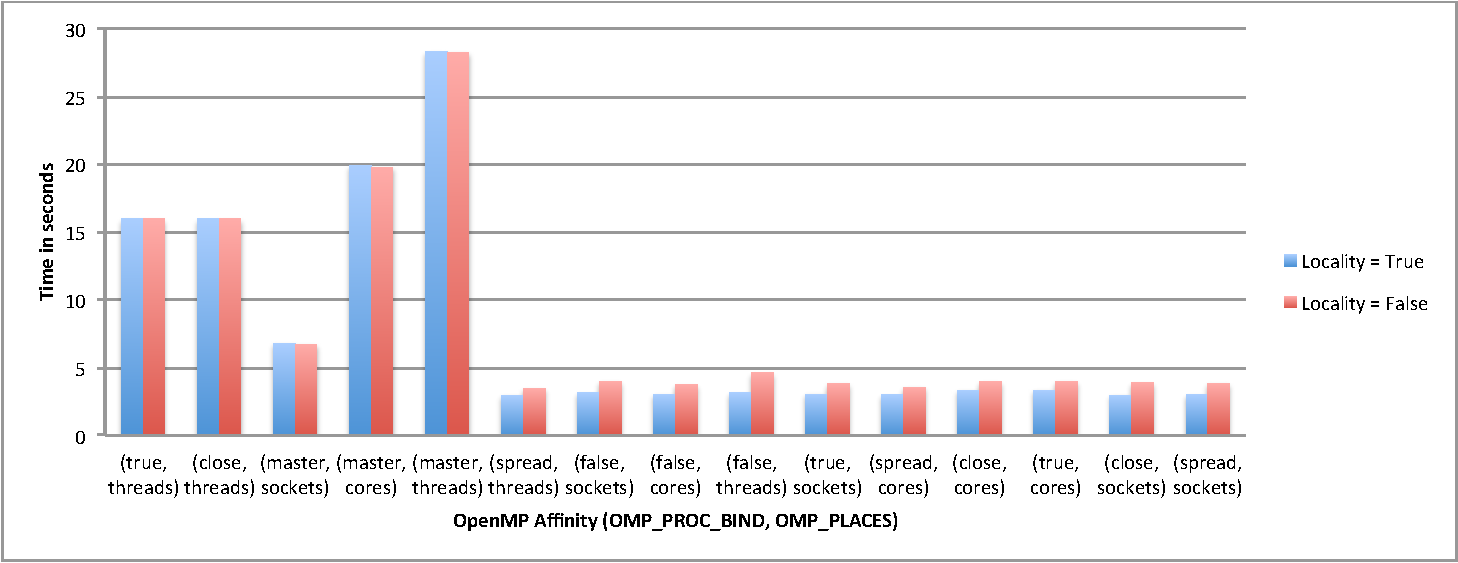
\includegraphics[height=0.4\textwidth, width=0.8\textwidth]{./Images/10Perf.pdf}
       \caption{Performance with 10 OpenMP threads on \textit{Crest}}
       \label{fig:10th}
\end{figure}
%
 We experiment with the locality aware and locality unaware versions of the Jacobi program along with the default first-touch policy to observe the behavior over varying number of threads. 
 For each thread count we record the POWER8 hardware counters and the placement of the threads on the hardware. 
 Figure ~\ref{fig:10th} and ~\ref{fig:20th} shows the performance of 10 and 20 OpenMP threads with different OpenMP Affinity settings respectively. We observed similar results for 40, 80 and 160 OpenMP threads and hence do not show them here.
%
\begin{figure}[h!]
  \centering
  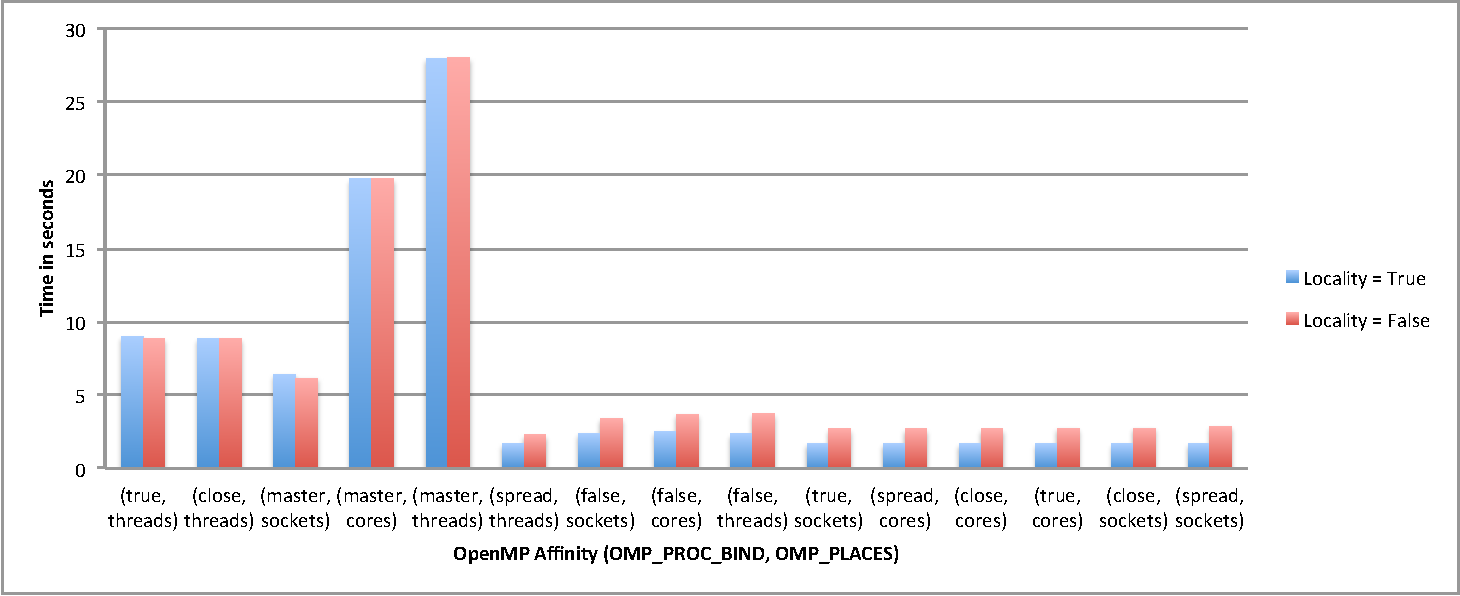
\includegraphics[height=0.4\textwidth, width=0.8\textwidth]{./Images/20Perf.pdf}
       \caption{Performance with 20 OpenMP threads on \textit{Crest}}
       \label{fig:20th}
\end{figure}
%
\begin{figure}[h!]
  \centering
  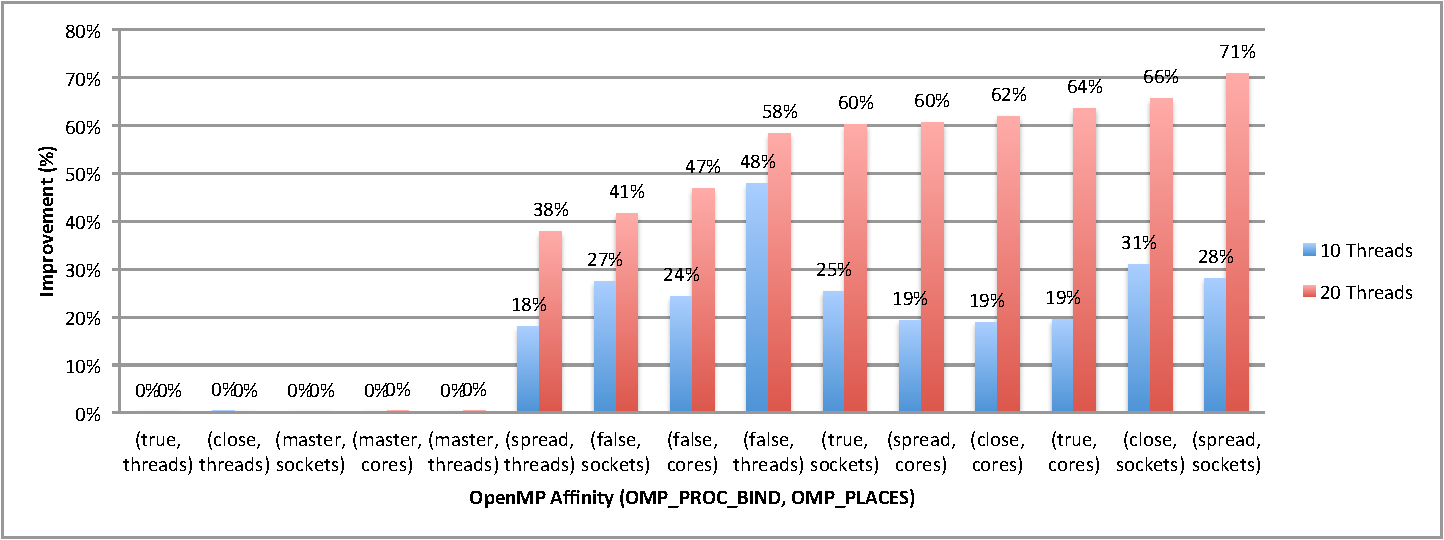
\includegraphics[height=0.4\textwidth, width=0.8\textwidth]{./Images/PerfI.pdf}
       \caption{Comparing Performance Improvement between different number of OpenMP threads}
       \label{fig:imp}
\end{figure}
From the data gathered we observe a similar trend for both 10 and 20 threads. 
For the \textit{(master, threads)} configuration all threads execute on CPUID 0. 
All threads execute in the same core as the master when the configuration is set to \textit{(master, core)}, similarly for \textit{(master, socket)} all threads execute in the same socket. In this case all threads are executing on CPUs 0 through 79 which corresponds to a single NUMA domain. When OMP\_PROC\_BIND set to master we see in Figure ~ref{fig:Imp} that there is no improvement of locality aware algorithms over non-locality aware algorithms (both using the first-touch policy).
For \textit{(close, threads)}, we observe that all OpenMP threads execute on random CPUs between 0-19. All of these cases don't suffer from memory locality issues because they access memory local to the memory within the chip.
In the \textit{(spread, sockets)} and \textit{(close, sockets)} configuration threads are spread across sockets but may be mapped to the same core. We observed that the \textit{(true, threads)} configuration is equivalent to the \textit{(close,threads)} according to the thread mappings.
For all OpenMP affinity settings  with OMP\_PROC\_BIND set to false, threads can migrate and are not bound to a specific thread, core or socket. This migration makes it less impactful on the data placement, but suffers from performance.